
\begin{frame}{Aplicación para Pase de Lista (1)}
\begin{block}{Motivación} 
Es necesario una herramienta que permita al profesor pasar asistencia de manera ágil y rápida. 
\begin{itemize}
\item El profesor debe ingresar los grupos a partir de archivos de texto
\item El profesor ingresa a pase de lista y selecciona uno de sus grupos
\item Puede seleccionar asistencia a todos o falta a todos para agilizar el proceso
\item La aplicacion genera un informe con las estadisticas de asistencias, faltas y retartdos
\item Originalmente la lista se manejaba por archivos de texto, despues se migró a una base de datos SQLite
\end{itemize}
\end{block} 
\end{frame}


\begin{frame}{Aplicación para Pasar Lista (2)}
%\begin{block}{Pantallas Principales} 
\begin{center}
	\begin{tabular}{cccc}
		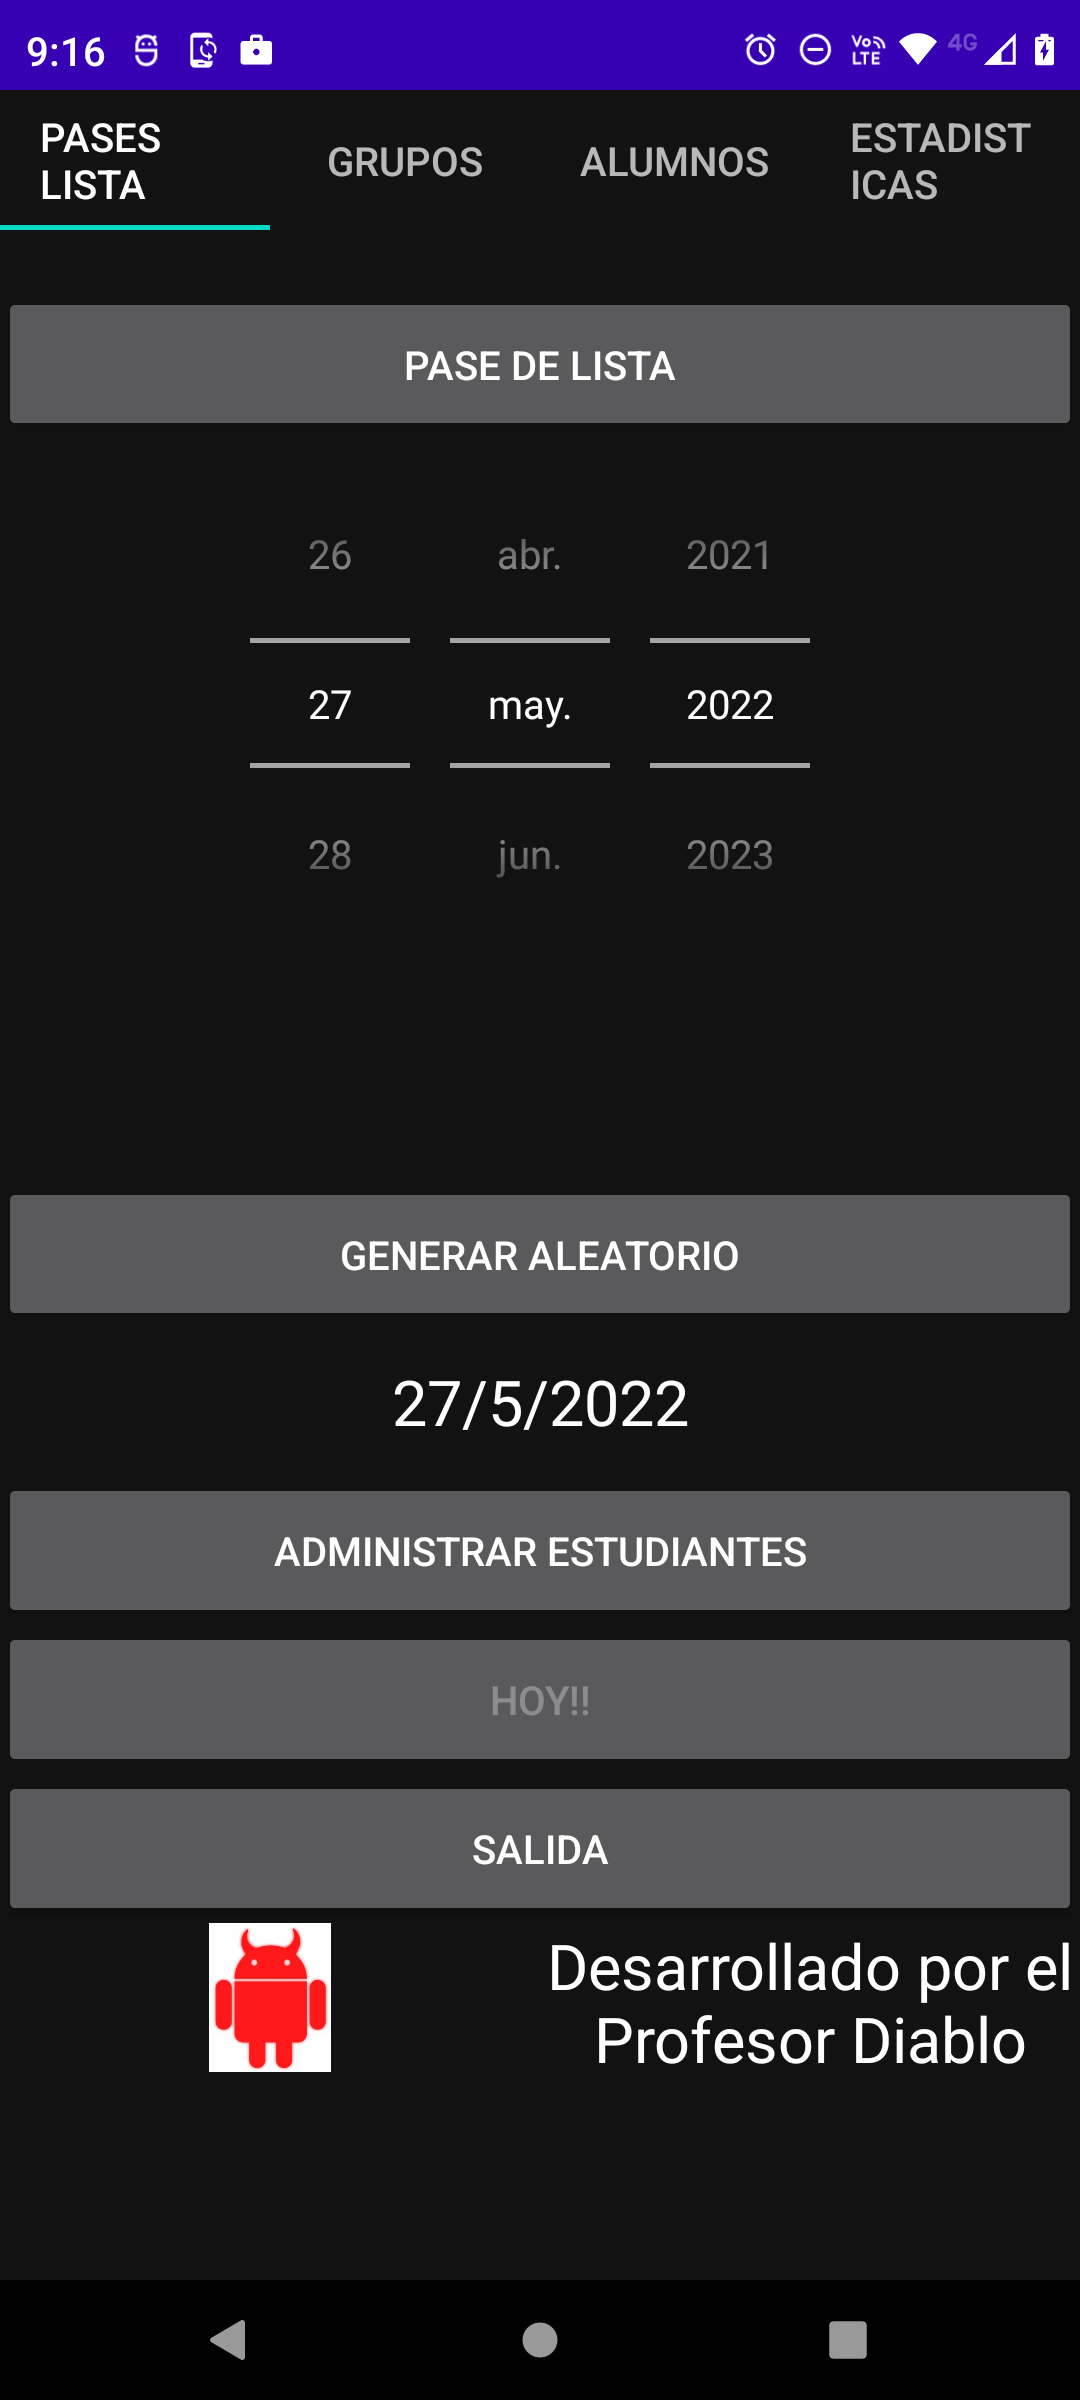
\includegraphics[width=0.20\linewidth]{2022_AppPaseLista/figs/PaseLista0.png} &
		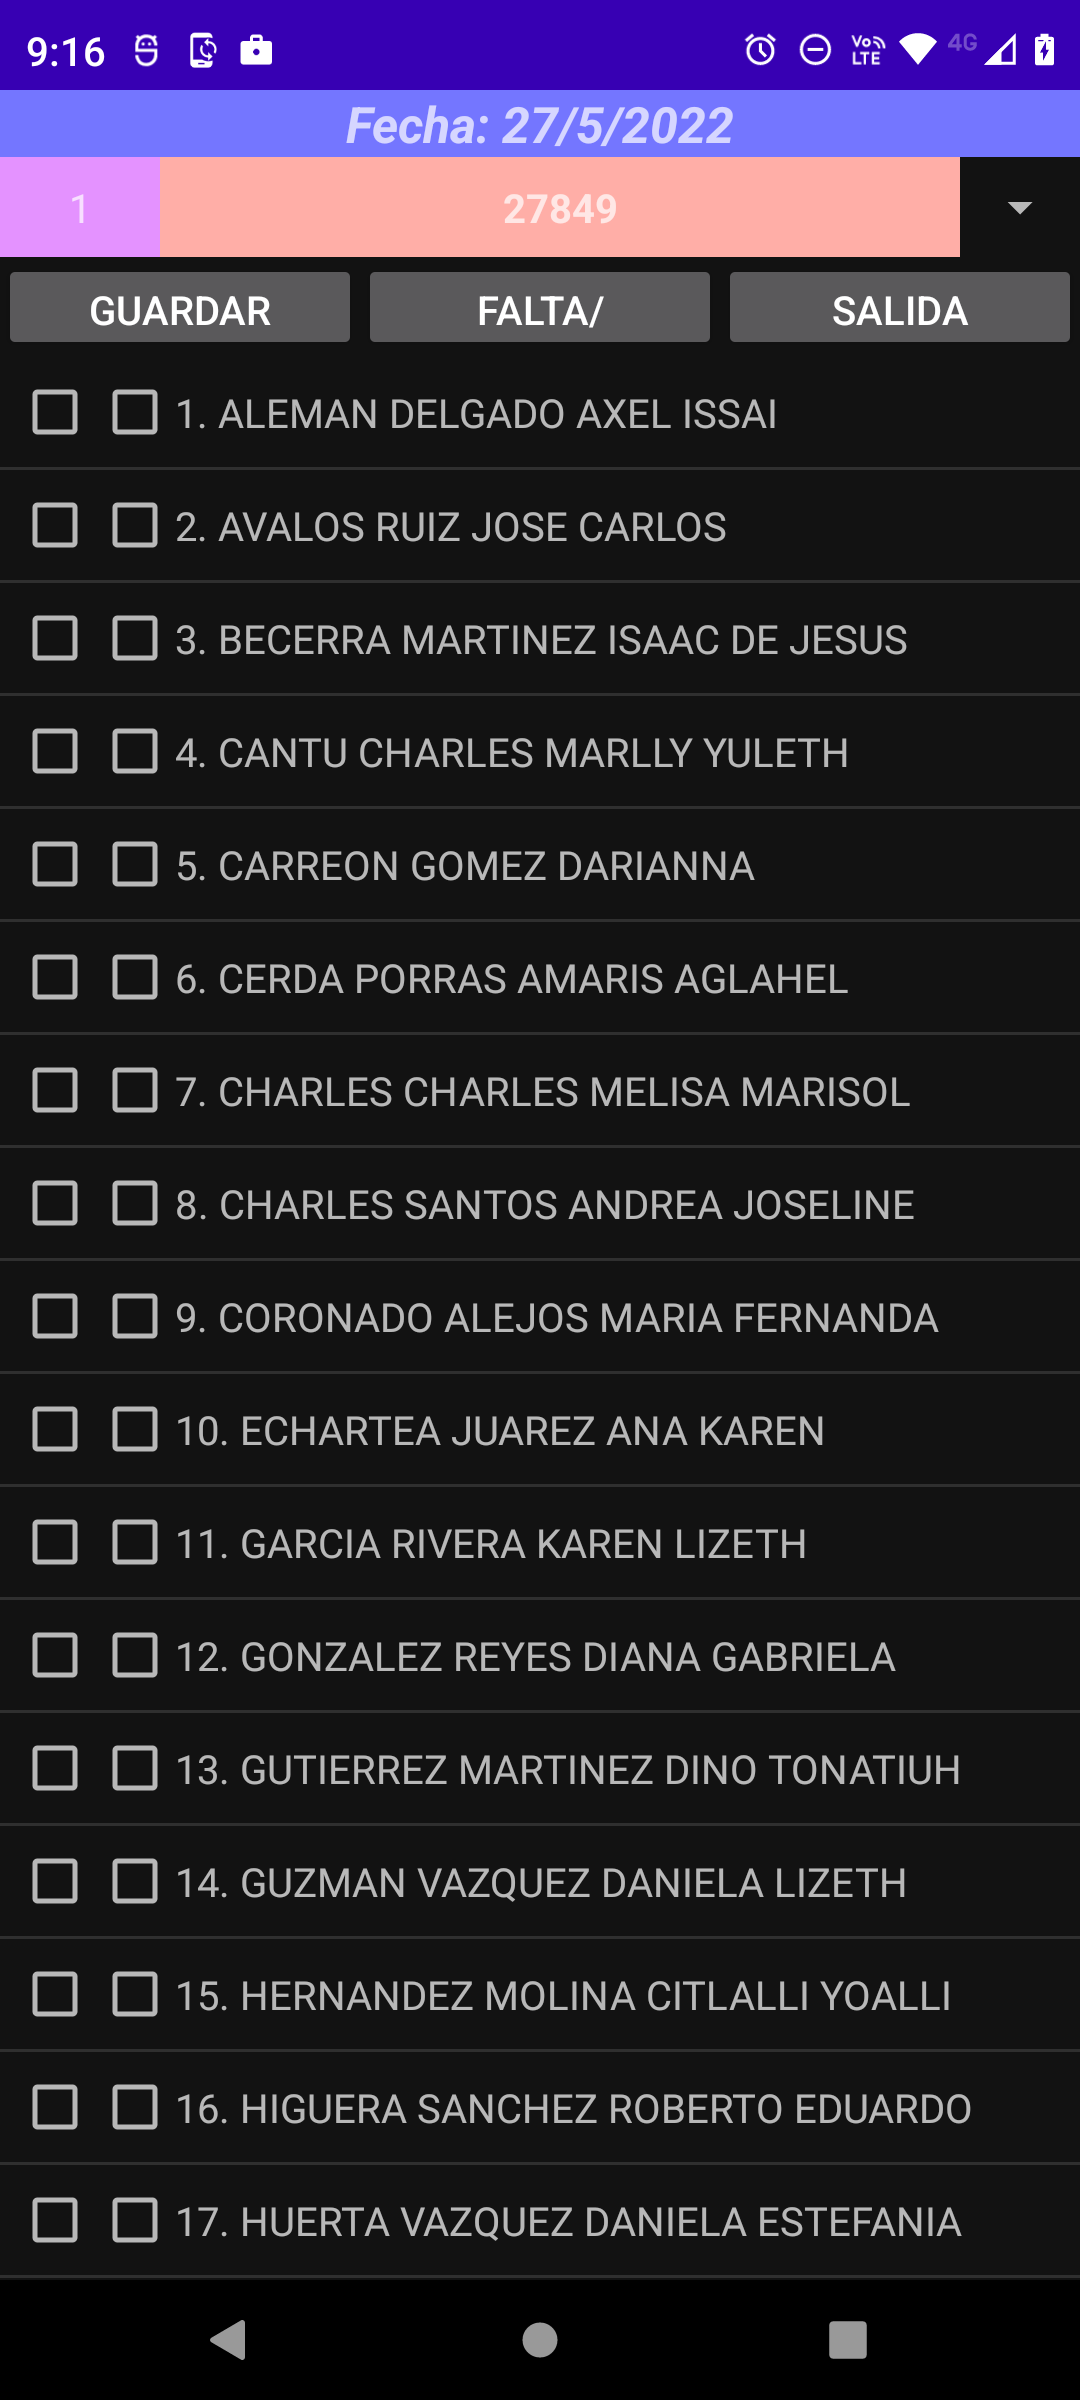
\includegraphics[width=0.20\linewidth]{2022_AppPaseLista/figs/PaseLista1.png} & 		 		
		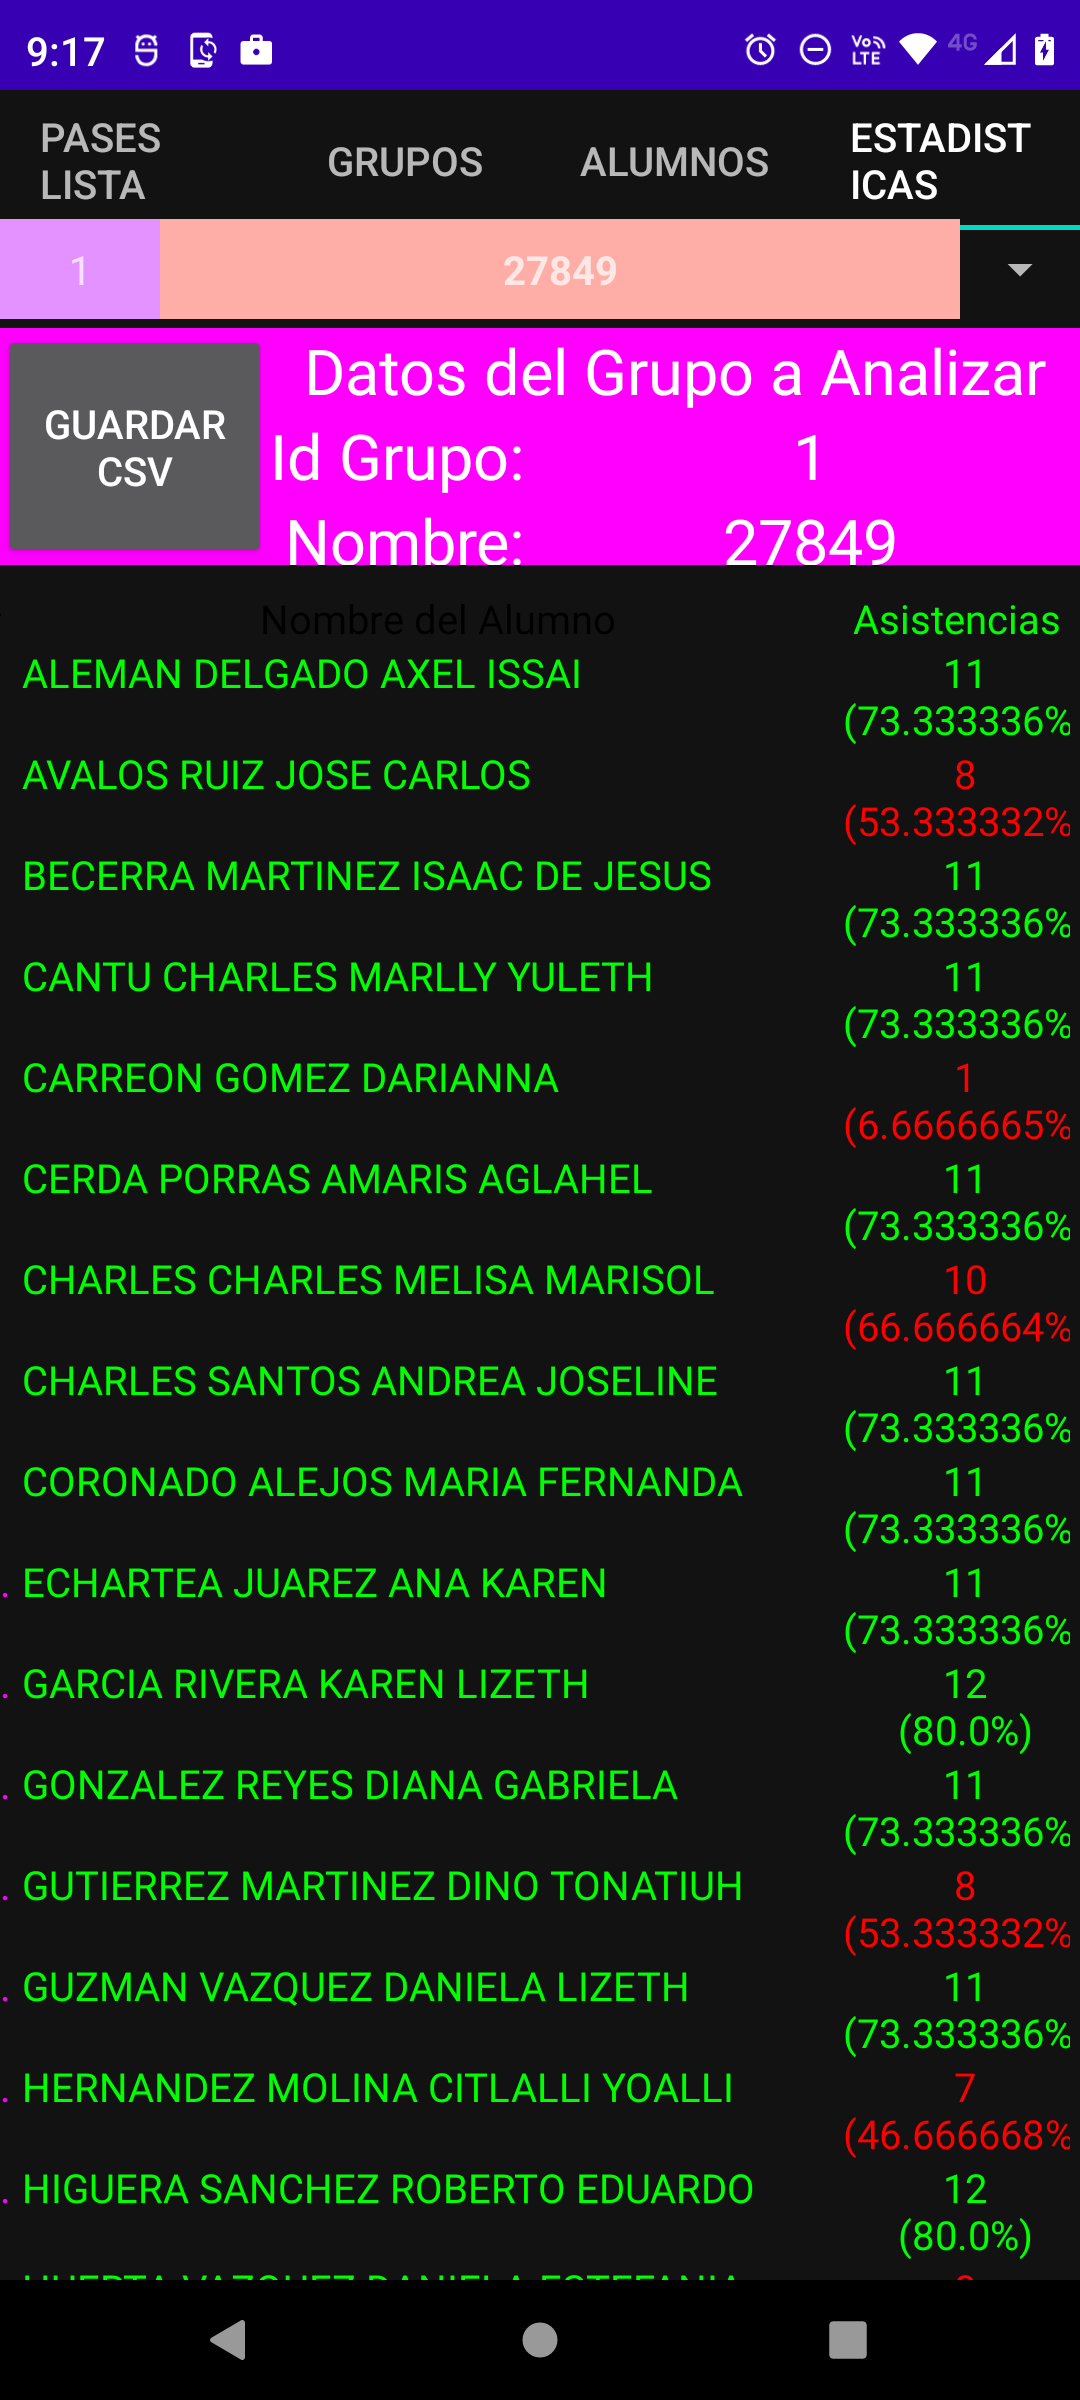
\includegraphics[width=0.20\linewidth]{2022_AppPaseLista/figs/PaseLista2.png} & 		
		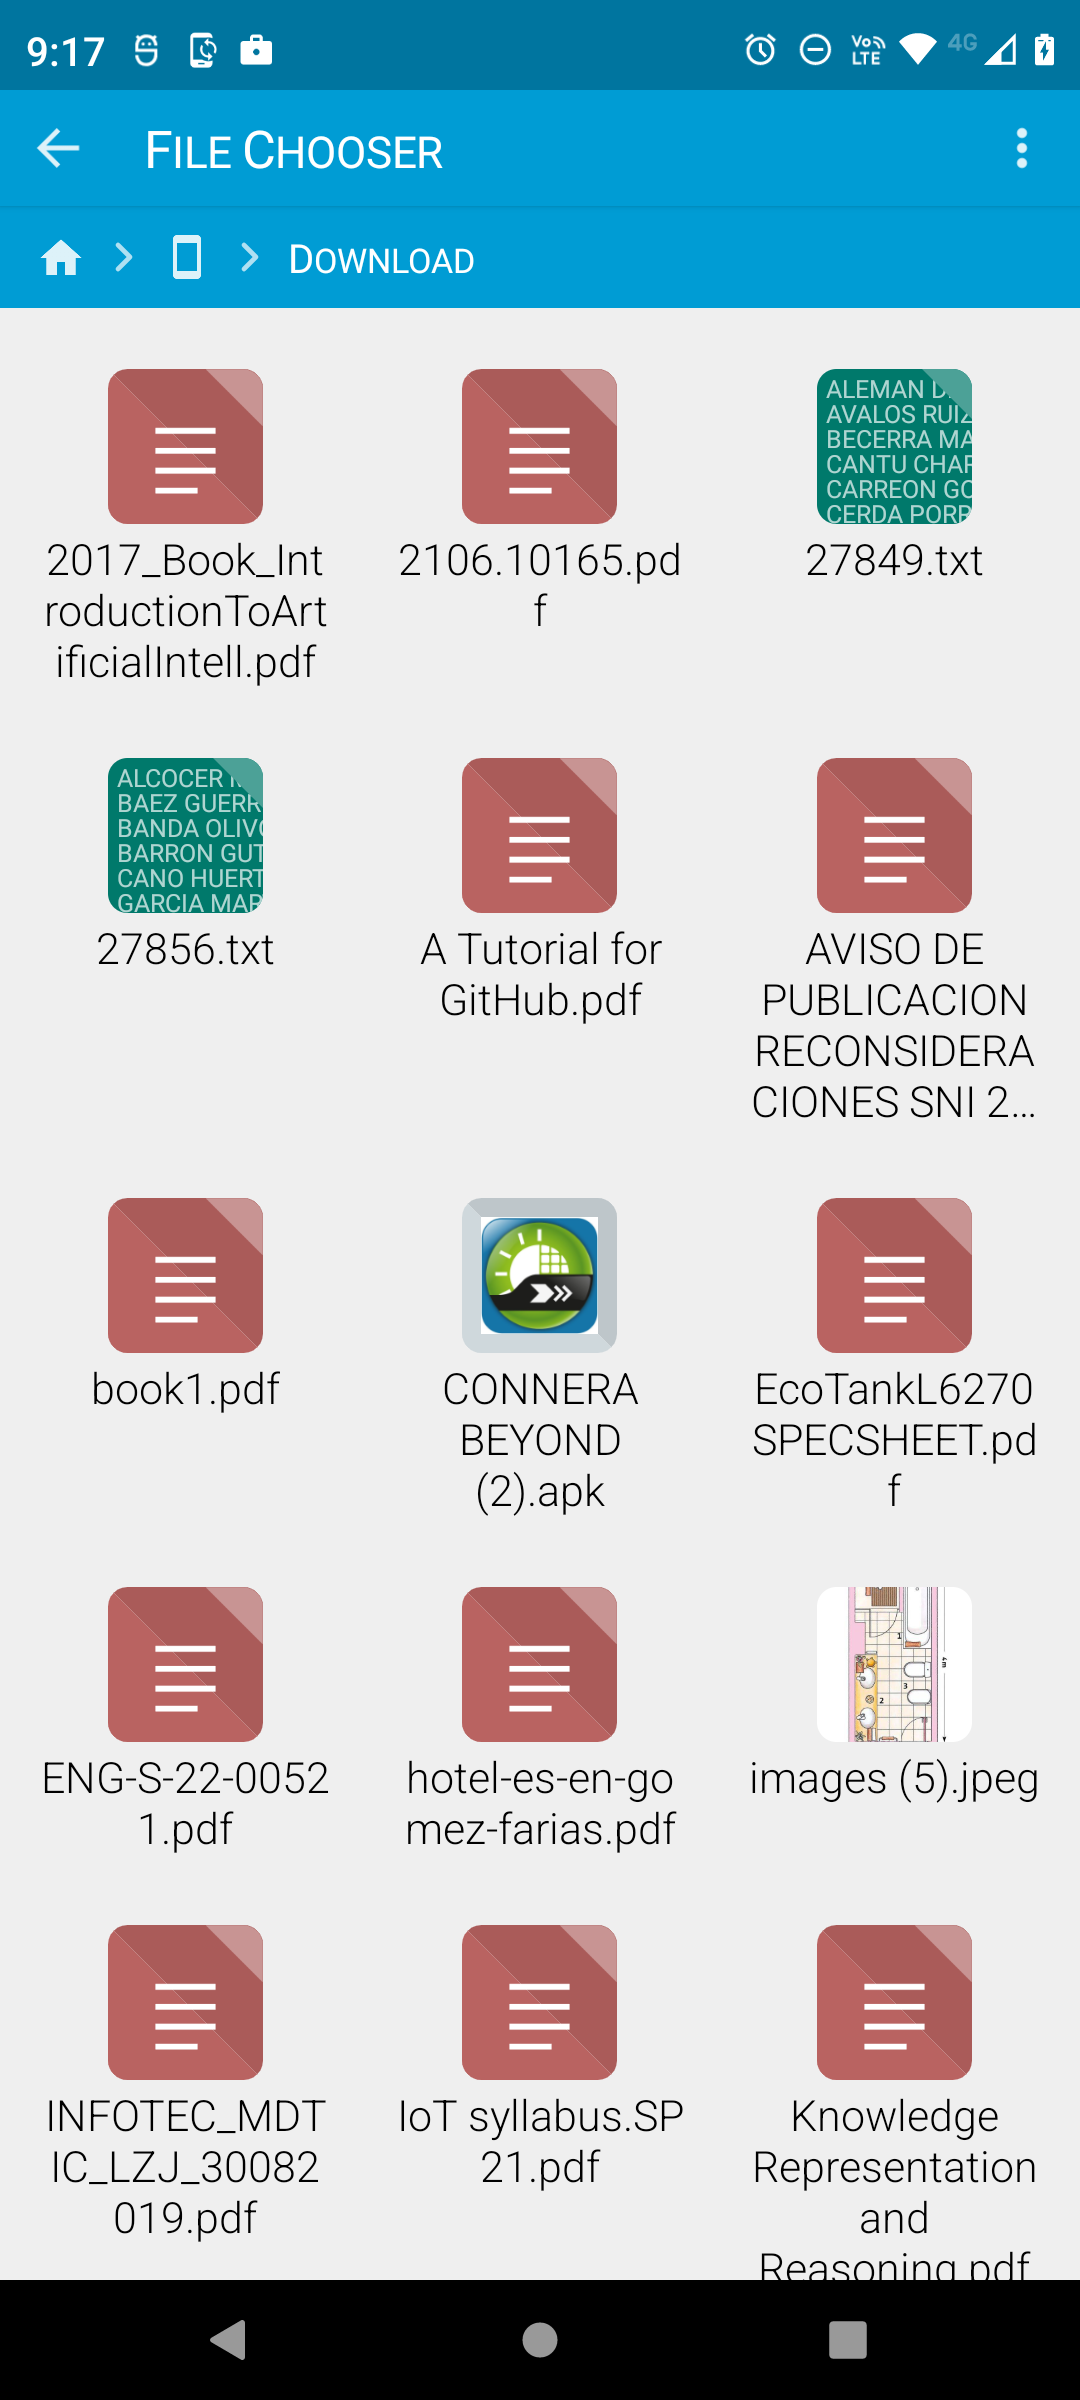
\includegraphics[width=0.20\linewidth]{2022_AppPaseLista/figs/PaseLista3.png} \\
	\end{tabular}
\end{center}
\end{frame}



